The \texttt{\pkglnk{model.term}} package contains the classes used by the application to
represent lambda terms and provides means for operating on them.

Lambda terms are represented as a tree structure of immutable objects
implementing the interface \texttt{\lnk{LambdaTerm}}. There are four types that
directly model their corresponding entities in the untyped lambda calculus:
\texttt{\lnk{Abstraction}}, \texttt{\lnk{Application}}, \texttt{\lnk{BoundVariable}} and
\texttt{\lnk{FreeVariable}}. For abstractions, the preferred name for the variable is stored.
Bound variables refer to their corresponding abstraction using De Bruijn indices.
Additionally, there are two more types that do not have
a direct counterpart in untyped lambda calculus: \texttt{\lnk{NamedTerm}} and
\texttt{\lnk{PartialApplication}}.

\texttt{\lnk{NamedTerm}} is a lambda term that has been assigned a name, either by a
library or by the user. In some cases (for instance when considered by a
reduction order polcy) it should be treated exactly like the term it
represents. In other cases (for instance when displaying the term) it should be
treated differently.

\texttt{\lnk{PartialApplication}} represents a series of nested applications, with
the left hand side of the innermost application being a named term that stands
for a library function (which is a series of nested abstractions). An
application where the left hand side is a partial application can be
transformed into a larger partial application. When the partial application
has collected as many arguments as the library function its inner named
term represents, it will be evaluated in one step and replaced by a lambda
term for its result. The purpose of this is to be able to accelerate large
computations involving numbers.

Except for testing for equality, all operations on lambda terms are carried out
by visitors. In addition to the universal \texttt{\lnk{Visitor}<T>} interface, which
is implemented by visitors carrying out an operation and returning a result of type
\texttt{T}, there are several abstract classes implementing this interface to make
typical operations on lambda terms easier. \texttt{\lnk{NameAgnosticVisitor}<T>} is a
visitor that ignores the names of terms (such as reduction orders),
\texttt{\lnk{ResolvedNamesVisitor}<T>} provides non-colliding names for variable names
used in abstractions and is intended for visitors displaying lambda terms, and
\texttt{\lnk{TermTransformer}} allows transforming a lambda term into a new term while
automatically removing the name tag from lambda terms that have been changed by
the transformation. It is intended for substitution operations and $\beta$-reductions.

\begin{figure}[H]
	\centering
	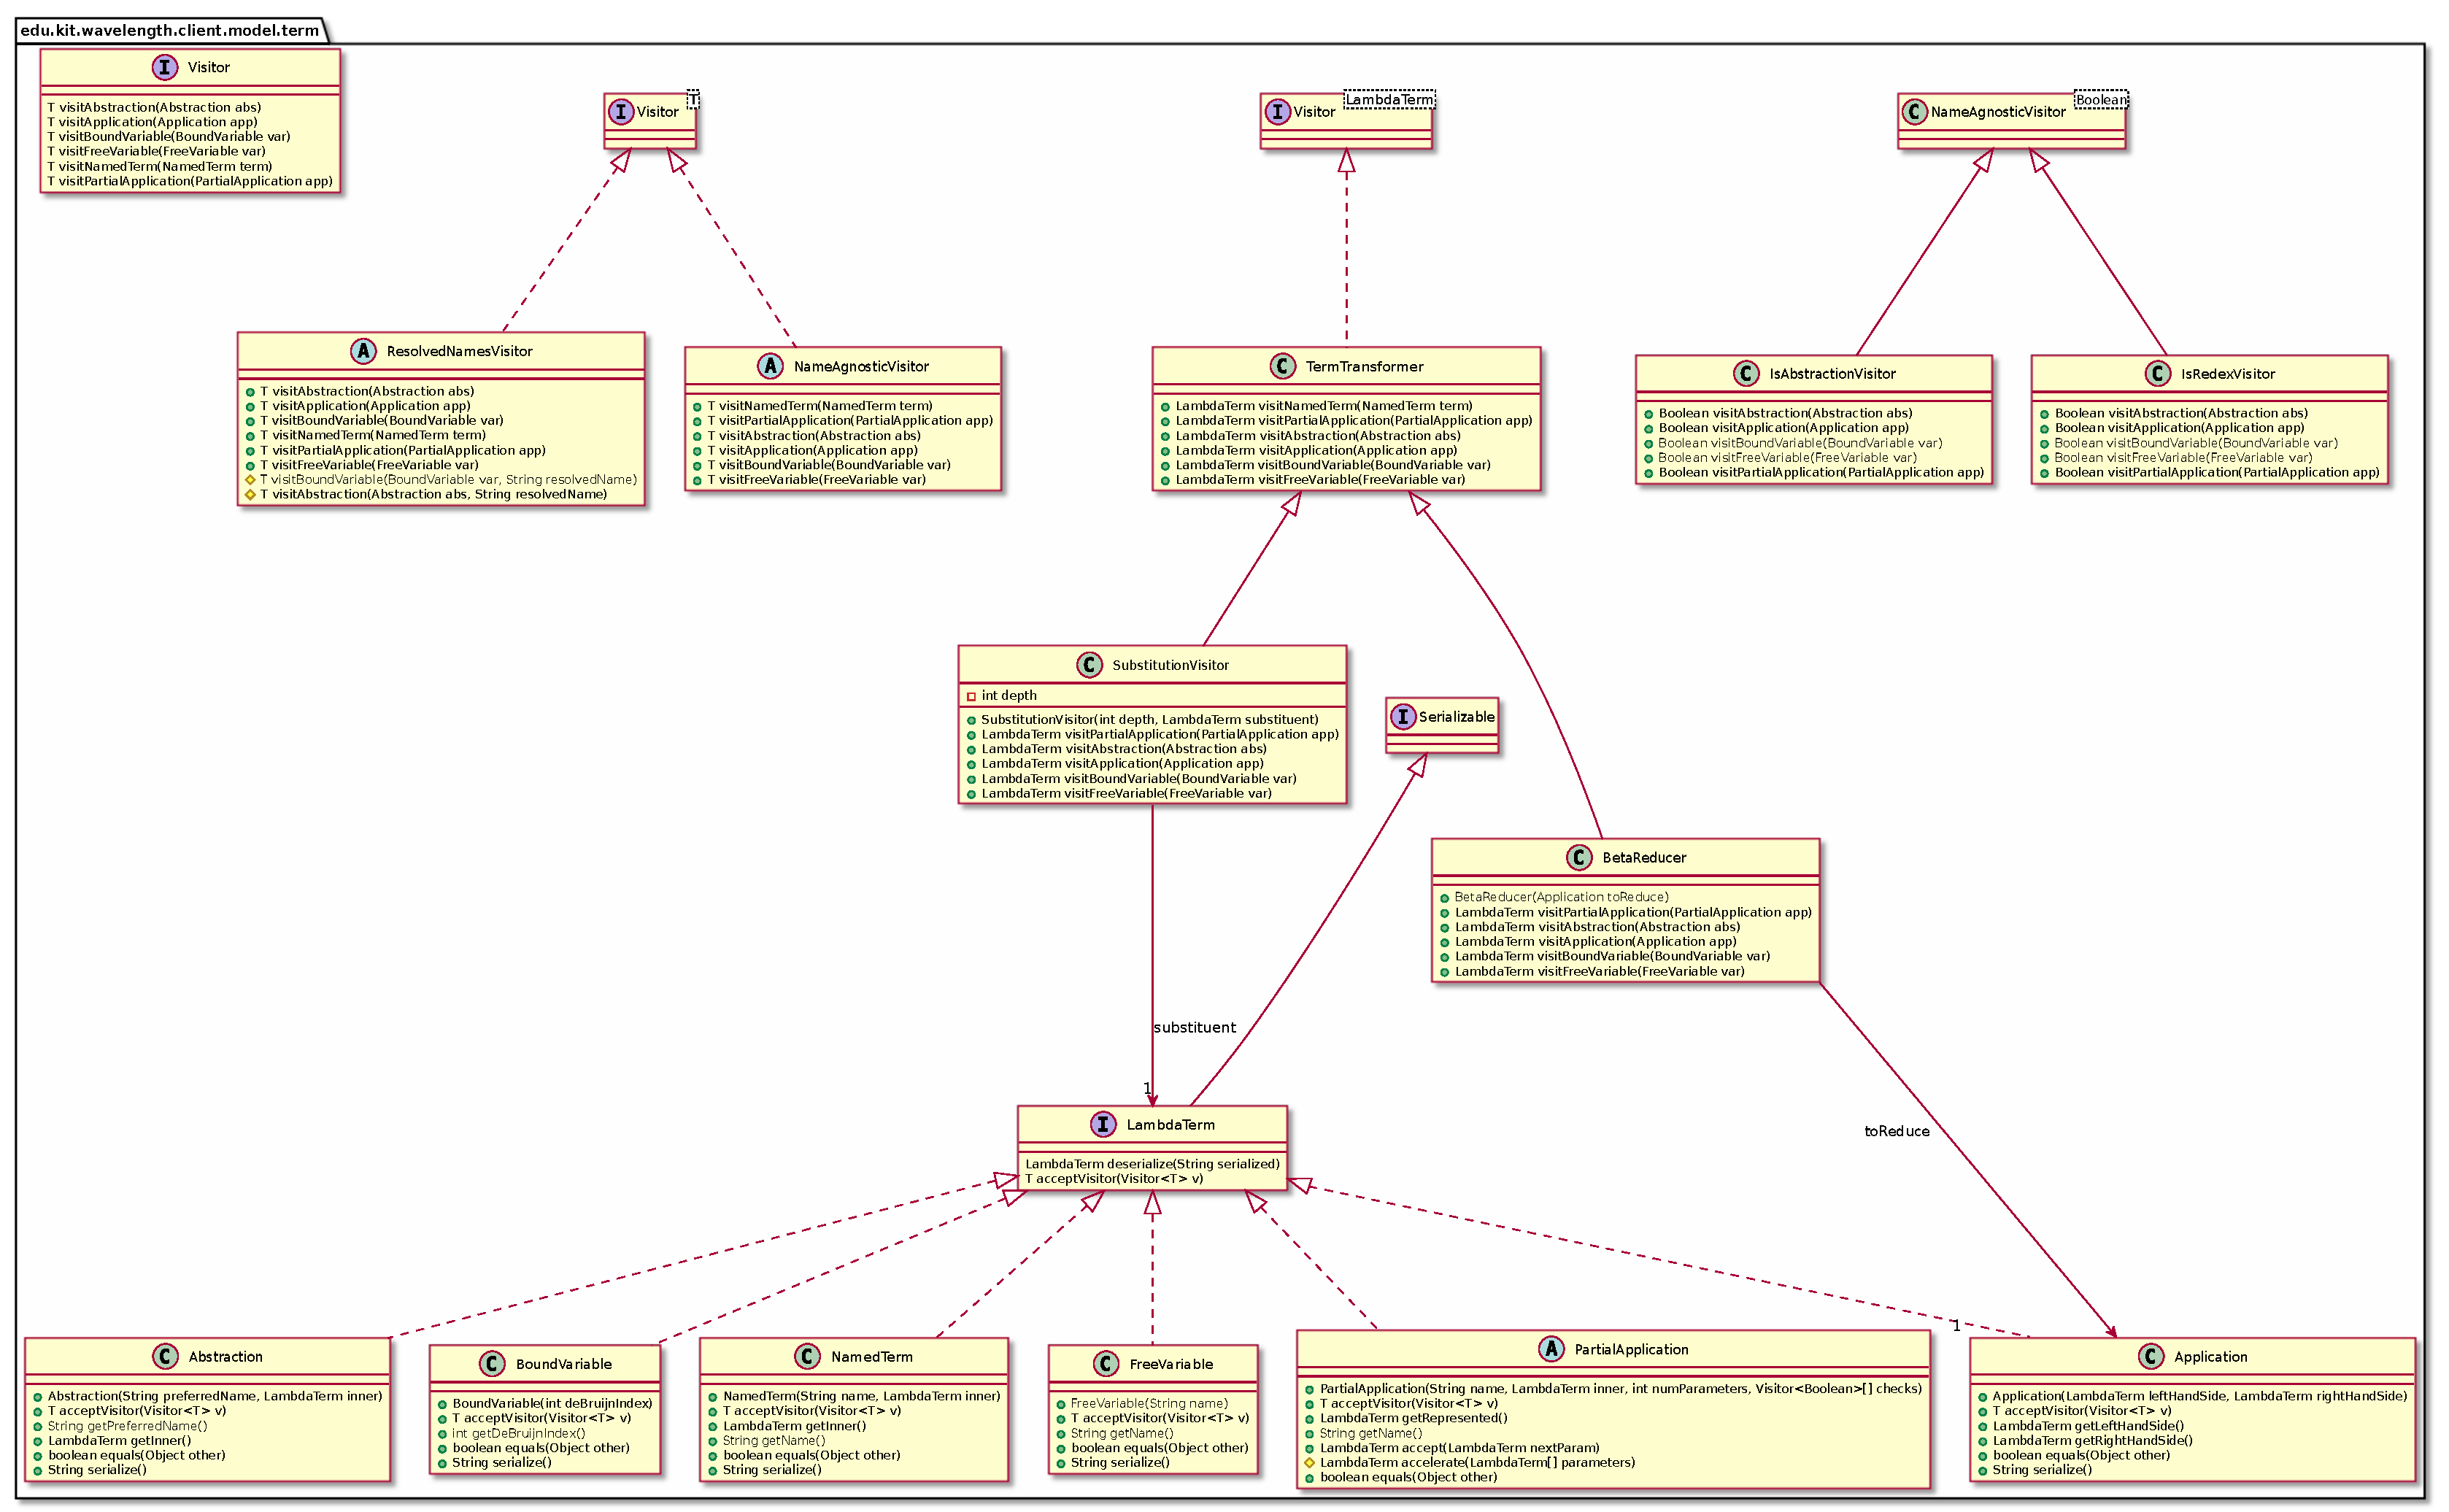
\includegraphics[width=\textwidth]{packageDiagrams/termPackage}
\end{figure}